\section{Linear algebra}

\subsection{What are matrices and what can we do with them?}

Similar to a two-dimensional array, a \textit{matrix} consists of real numbers arranged into \(m\) rows and \(n\) columns. Each real number is called an \textit{element} of the matrix, and the matrix is said to have an order of \(m \times n\). For example, the matrix below has the order \(3 \times 4\).
%
\[
\begin{pmatrix}
    1 & 8 & 3 & 4\\
    2 & 2 & 7 & 4\\
    -3 & 18 & 5 & 6
\end{pmatrix}
\]

Different names are given to matrices with special properties, as illustrated below.
%
\begin{itemize}
    \item A \textit{row matrix} is a matrix that has only one row.
    %
    \[
        \begin{pmatrix}
        1 & 2 & 3
        \end{pmatrix}
    \]
    
    \item A \textit{column matrix} is a matrix that has only one column.
    %
    \[
        \begin{pmatrix}
        1 \\ 2 \\ 3
        \end{pmatrix}
    \]
    
    \item A \textit{zero matrix}, denoted as \(0\), is a matrix where all elements are zero.
    %
    \[
        \begin{pmatrix}
            0 & 0 & 0 & 0\\
            0 & 0 & 0 & 0\\
            0 & 0 & 0 & 0
        \end{pmatrix}
    \]
    
    \item A \textit{square matrix} is a matrix with the same number of rows and columns.
    %
    \[
        \begin{pmatrix}
            1 & 2 & 3\\
            4 & 5 & 6\\
            7 & 8 & 9
        \end{pmatrix}
    \]
    
    \item In a square matrix, the diagonal connecting the top left element and the bottom right element is called the \textit{principal diagonal} (highlighted in red below). If the elements not lying on the principal diagonal are all zero, then the matrix called is a \textit{diagonal matrix}.
    %
    \[
        \begin{pmatrix}
            {\color{BrickRed} 1} & 0 & 0\\
            0 & {\color{BrickRed} 2} & 0\\
            0 & 0 & {\color{BrickRed} 3}
        \end{pmatrix}
    \]

    \item In a diagonal matrix of order \(n \times n\), if all principal diagonal elements are 1, then the matrix is an identity matrix. Such a matrix is denoted as either \(I_n\) or \(I\).
    %
    \[
        I_3 = 
        \begin{pmatrix}
            1 & 0 & 0\\
            0 & 1 & 0\\
            0 & 0 & 1
        \end{pmatrix}
    \]
\end{itemize}

Matrices of the same order can be added and subtracted element-by-element. To multiply a matrix by a scalar \(k\), simply multiply all elements in the matrix by \(k\).
%
\begin{align*}
\begin{pmatrix}
    3 & 9\\
    6 & 7
\end{pmatrix}
+
\begin{pmatrix}
    7 & 4\\
    3 & 1
\end{pmatrix}
&=
\begin{pmatrix}
    10 & 13\\
    9 & 8
\end{pmatrix}\\
%--------------------
\begin{pmatrix}
    3 & 9\\
    6 & 7
\end{pmatrix}
-
\begin{pmatrix}
    7 & 4\\
    3 & 1
\end{pmatrix}
&=
\begin{pmatrix}
    -4 & 5\\
    3 & 6
\end{pmatrix}\\
%--------------------
3 \times
\begin{pmatrix}
    3 & 9\\
    6 & 7
\end{pmatrix}
&=
\begin{pmatrix}
    9 & 27\\
    18 & 21
\end{pmatrix}
\end{align*}

Matrices can be multiplied together to give another matrix.
%
\[
\begin{pmatrix}
    3 & 9\\
    6 & 8
\end{pmatrix}
+
\begin{pmatrix}
    7 & 4\\
    2 & 1
\end{pmatrix}
=
\begin{pmatrix}
    3\times 7 + 9\times 2 & 3\times 4 + 9\times 1\\
    6\times 7 + 8\times 2 & 6\times 4 + 8\times 1
\end{pmatrix}
=
\begin{pmatrix}
    39 & 21\\
    58 & 32
\end{pmatrix}
\]
%
Note, however, that matrix multiplication is not commutative. In general, we have \(AB \neq BA\) for two matrices \(A\) and \(B\).

A square matrix can be raised to an integer power \(k\) through repeated multiplication.
%
\[
\begin{pmatrix}
    1 & 2\\
    3 & 4
\end{pmatrix}^3
=
\begin{pmatrix}
    1 & 2\\
    3 & 4
\end{pmatrix}
\begin{pmatrix}
    1 & 2\\
    3 & 4
\end{pmatrix}
\begin{pmatrix}
    1 & 2\\
    3 & 4
\end{pmatrix}
\]
%
A diagonal matrix can be raised to an integer power \(k\) simply by raising each of its elements to the power \(k\).


\subsection{Determinants and how to compute them}

For any square matrix \(A\), we can compute its determinant, which is a scalar denoted as either \(\abs{A}\) or \(\det{\;A}\).


\subsubsection{Determinant of a \(2 \times 2\) matrix}\label{sec:determinant-2x2}

The determinant of a \(2 \times 2\) matrix can be calculated using the following formula. See figure \ref{fig:Ch11-det-2x2}.
%
\[
\begin{vmatrix}
    a_{11} & a_{12}\\
    a_{21} & a_{22}
\end{vmatrix}
%
= a_{11}a_{22} - a_{12}a_{21}
\]

\begin{figure}[H]
    \centering
    \includegraphics[width=0.15\linewidth]{Images/Ch11/Det2x2.png}
    \caption{Computing the determinant of a \(2\times2\) matrix.}
    \label{fig:Ch11-det-2x2}
\end{figure}



\subsubsection{Determinant of a \(3 \times 3\) matrix}

The determinant of a \(3 \times 3\) matrix can be calculated using the formula below. See figure \ref{fig:Ch11-det-3x3}.
%
\[
\begin{vmatrix}
    a_{11} & a_{12} & a_{13}\\
    a_{21} & a_{22} & a_{23}\\
    a_{31} & a_{32} & a_{33}
\end{vmatrix}
= a_{11}a_{22}a_{33} + a_{12}a_{23}a_{31} + a_{13}a_{21}a_{32} - a_{13}a_{22}a_{31} - a_{11}a_{23}a_{32} - a_{12}a_{21}a_{33}
\]


\begin{figure}[H]
    \centering
    \includegraphics[width=0.4\linewidth]{Images/Ch11/Det3x3.png}
    \caption{Computing the determinant of a \(3\times3\) matrix.}
    \label{fig:Ch11-det-3x3}
\end{figure}



\subsubsection{Determinant of a \(4 \times 4\) matrix}

Given a \(4\times 4\) matrix:
%
\[
A =
%
\begin{pmatrix}
    a_{11} & a_{12} & a_{13} & a_{14}\\
    a_{21} & a_{22} & a_{23} & a_{24}\\
    a_{31} & a_{32} & a_{33} & a_{34}\\
    a_{41} & a_{42} & a_{43} & a_{44}
\end{pmatrix}
\]
%
we compute its determinant by breaking it down into a series of \(3 \times 3\) matrices.
%
\begin{align*}
    \abs{A} =\;& + a_{11} \cdot \abs{A_{11}}\\
    & - a_{12} \cdot \abs{A_{12}}\\
    & + a_{13} \cdot \abs{A_{13}}\\
    & -  a_{14} \cdot \abs{A_{14}}
\end{align*}
%
where \(A_{ij}\) denotes the submatrix obtained by deleting the \(i\)-th row and \(j\)-th column from \(A\). An example is shown below.
%
\begin{align*}
&\; \begin{vmatrix}
2 & 1 & 0 & 3\\
4 & -1 & 2 & 0\\
-3 & 2 & 1 & 5\\
1 & 0 & -2 & 3
\end{vmatrix}\\
%
=&
%
2 \cdot
\begin{vmatrix}
-1 & 2 & 0\\
2 & 1 & 5\\
0 & -2 & 3
\end{vmatrix}
- 1 \cdot 
\begin{vmatrix}
4 & 2 & 0\\
-3 & 1 & 5\\
1 & -2 & 3
\end{vmatrix}
+ 0 \cdot 
\begin{vmatrix}
4 & -1 & 0\\
-3 & 2 & 5\\
1 & 0 & 3
\end{vmatrix}
- 3 \cdot
\begin{vmatrix}
4 & -1 & 2\\
-3 & 2 & 1\\
1 & 0 & -2
\end{vmatrix}\\
%
=& 2\cdot(-25) - 1\cdot 80 + 0 - 3\cdot (-15)\\
=& -50 - 80 + 0 - (-45)\\
=& -85
\end{align*}




\subsubsection{Leibniz formula for determinants}

Let's review the formula used for computing the determinant of a \(3 \times 3\) matrix. This time, our aim is to create a more elegant and concise representation of this formula that can be generalised to square matrices of any order.

To begin with, we highlight the subscript of each element like so.
%
\begin{align}
&\;
\begin{vmatrix}
    a_{11} & a_{12} & a_{13}\\
    a_{21} & a_{22} & a_{23}\\
    a_{31} & a_{32} & a_{33}
\end{vmatrix} \notag \\
%
=&\; a_{{\color{BrickRed}1}{\color{MidnightBlue}1}}
a_{{\color{BrickRed}2}{\color{MidnightBlue}2}}
a_{{\color{BrickRed}3}{\color{MidnightBlue}3}} + 
%
a_{{\color{BrickRed}1}{\color{MidnightBlue}2}}
a_{{\color{BrickRed}2}{\color{MidnightBlue}3}}
a_{{\color{BrickRed}3}{\color{MidnightBlue}1}} + 
%
a_{{\color{BrickRed}1}{\color{MidnightBlue}3}}
a_{{\color{BrickRed}2}{\color{MidnightBlue}1}}
a_{{\color{BrickRed}3}{\color{MidnightBlue}2}} - 
%
a_{{\color{BrickRed}1}{\color{MidnightBlue}3}}
a_{{\color{BrickRed}2}{\color{MidnightBlue}2}}
a_{{\color{BrickRed}3}{\color{MidnightBlue}1}} - 
%
a_{{\color{BrickRed}1}{\color{MidnightBlue}1}}
a_{{\color{BrickRed}2}{\color{MidnightBlue}3}}
a_{{\color{BrickRed}3}{\color{MidnightBlue}2}} - 
%
a_{{\color{BrickRed}1}{\color{MidnightBlue}2}}
a_{{\color{BrickRed}2}{\color{MidnightBlue}1}}
a_{{\color{BrickRed}3}{\color{MidnightBlue}3}}
\label{eq:3x3-determinant-highlighted}
\end{align}
%
We note that in each of the six terms in \eqref{eq:3x3-determinant-highlighted}, the relationship between the red and blue subscripts can be viewed as a permutation in the symmetric group of degree 3.
%
\[
    S_3 = \left\{
    \begin{pmatrix}
        1 & 2 & 3\\
        1 & 2 & 3
    \end{pmatrix},
    %
    \begin{pmatrix}
        1 & 2 & 3\\
        1 & 3 & 2
    \end{pmatrix},
    %
    \begin{pmatrix}
        1 & 2 & 3\\
        2 & 1 & 3
    \end{pmatrix},
    %
    \begin{pmatrix}
        1 & 2 & 3\\
        2 & 3 & 1
    \end{pmatrix},
    %
    \begin{pmatrix}
        1 & 2 & 3\\
        3 & 1 & 2
    \end{pmatrix},
    %
    \begin{pmatrix}
        1 & 2 & 3\\
        3 & 2 & 1
    \end{pmatrix}
    \right\}
\]
%
For example, the last term \(a_{{\color{BrickRed}1}{\color{MidnightBlue}2}}
a_{{\color{BrickRed}2}{\color{MidnightBlue}1}}
a_{{\color{BrickRed}3}{\color{MidnightBlue}3}}\) corresponds to the permutation \(
\begin{pmatrix}
    {\color{BrickRed}1} & {\color{BrickRed}2} & {\color{BrickRed}3}\\
    {\color{MidnightBlue}2} & {\color{MidnightBlue}1} & {\color{MidnightBlue}3}
\end{pmatrix}
\).

This gives us the following (incomplete) formula:
%
\[\abs{A} = \sum_{\sigma \in S_n} \left( \boxed{\text{\textbf{?}}} \cdot \prod_{i = 1}^n a_{i, \sigma(i)}\right)\]
%
This is incomplete because we still have to figure out what function goes in the blank labelled \(\boxed{\text{\textbf{?}}}\). This function should return \(+1\) for the first three terms in \eqref{eq:3x3-determinant-highlighted} and \(-1\) for the last three terms.

As it turns out, there \textit{is} a function that does this job perfectly: the sign function, introduced in section \ref{sec:sign-of-permutation}. (As a reminder, the sign of a permutation can either be \(+1\) and \(-1\) depending on the parity of the number of disorders therein.) The complete formula is therefore as follows.
%
\[\abs{A} = \sum_{\sigma \in S_n} \left(  \prod_{i = 1}^n a_{i, \sigma(i)}\right)\]
%
This is known as the Leibniz formula for determinants and can be applied to squared matrices of any order.


\subsubsection{The determinant as the volume of a parallelopiped}

The determinant of a matrix can be interpreted geometrically.
%
A \(2\times2\) matrix can be thought of as an array of two column vectors, each of which has two elements. The absolute value of the matrix's determinant is equal to the area of the parallelogram formed between the two column vectors.

Similarly, a \(3\times3\) matrix can be viewed as an array of three column vectors, each with three elements. The absolute value of the matrix's determinant is equal to the volume of the parallelopiped formed between the three column vectors.
%
\begin{align*}
    \begin{pmatrix}
        a_{11} & a_{12}\\
        a_{21} & a_{22}
    \end{pmatrix}
    &\rightarrow
    \left\{
    \begin{pmatrix}
        a_{11} \\ a_{21}
    \end{pmatrix},
    \begin{pmatrix}
        a_{12} \\ a_{22}
    \end{pmatrix}
    \right\}\\
    \begin{pmatrix}
        a_{11} & a_{12} & a_{13}\\
        a_{21} & a_{22} & a_{23}\\
        a_{31} & a_{32} & a_{33}
    \end{pmatrix}
    &\rightarrow
    \left\{
    \begin{pmatrix}
        a_{11}\\
        a_{21}\\
        a_{31}
    \end{pmatrix},
    \begin{pmatrix}
        a_{12}\\
        a_{22}\\
        a_{32}
    \end{pmatrix},
    \begin{pmatrix}
        a_{13}\\
        a_{23}\\
        a_{33}
    \end{pmatrix}
    \right\}
\end{align*}

This is true for square matrices of any other order as well.




\subsubsection{Recursive method using upper triangular matrices}

A square matrix is called an \textit{upper triangular} matrix if all of its elements below the principal diagonal are zero. An example is displayed below.
%
\[
\begin{pmatrix}
    1 & 4 & 6 & 3\\
    {\color{BrickRed}0} & 4 & 1 & 5\\
    {\color{BrickRed}0} & {\color{BrickRed}0} & 9 & 2\\
    {\color{BrickRed}0} & {\color{BrickRed}0} & {\color{BrickRed}0} & 7
\end{pmatrix}
\]
%
An upper triangular matrix has the special property that its determinant must be equal to the product of the elements of its principal diagonal. (This can be easily verified using the Leibniz formula for determinants.) For instance, the matrix above has the determinant \(1 \times 4 \times 9 \times 7 = 252\).

How can we use this to find the determinant of \textit{any} square matrix? To do this let us introduce the following \textit{row operations}. Each row operation takes a matrix \(M\) and modifies it, outputting a new matrix \(M'\).
%
\begin{itemize}
    \item Add the product between a nonzero constant \(k\) and one of the rows to another row. The determinant of the matrix is conserved under this operation.
    %
    \begin{equation}
        \begin{pmatrix}
            1 & 2 & 3\\
            4 & 5 & 6\\
            7 & 8 & 9
        \end{pmatrix}
        \rightarrow
        \begin{pmatrix}
            1 & 2 & 3\\
            4 & 5 & 6\\
            0 & -6 & -12
        \end{pmatrix}
        \tag{\(R_3 \rightarrow R_3 - 7R_2\)}
    \end{equation}
    
    \item Multiply one of the rows by a nonzero constant \(k\). This multiplies the determinant by \(k\).
    %
    \begin{equation}
        \begin{pmatrix}
            1 & 2 & 3\\
            4 & 5 & 6\\
            7 & 8 & 9
        \end{pmatrix}
        \rightarrow
        \begin{pmatrix}
            2 & 4 & 6\\
            4 & 5 & 6\\
            7 & 8 & 9
        \end{pmatrix}
        \tag{\(R_1 \rightarrow 2R_1\)}
    \end{equation}
    
    \item Swap two of the rows. The negates the determinant of the matrix.
    %
    \begin{equation}
        \begin{pmatrix}
            1 & 2 & 3\\
            4 & 5 & 6\\
            7 & 8 & 9
        \end{pmatrix}
        \rightarrow
        \begin{pmatrix}
            4 & 5 & 6\\
            1 & 2 & 3\\
            7 & 8 & 9
        \end{pmatrix}
        \tag{Swap \(R_1\) and \(R_2\)}
    \end{equation}
\end{itemize}

These three row operations allow us to transform any given matrix \(M\) into an upper triangular matrix \(M'\). By computing \(\abs{M'}\) and keeping track of the sequence of operations used, we are able to work out the determinant of the original matrix \(M\). An example of this is given below.
%
\begin{align}
    A &=\;
    \begin{pmatrix}
        1 & 2 & 3\\
        4 & 5 & 6\\
        7 & 8 & 10
    \end{pmatrix}\notag\\
    %
    &\rightarrow
    \begin{pmatrix}
        1 & 2 & 3\\
        0 & -3 & -6\\
        7 & 8 & 10
    \end{pmatrix} \tag{\(R_2 \rightarrow R_2 - 4R_1\)}\\
    %
    &\rightarrow
    \begin{pmatrix}
        1 & 2 & 3\\
        0 & -3 & -6\\
        0 & -6 & -11
    \end{pmatrix} \tag{\(R_3 \rightarrow R_3 - 7R_1\)}\\
    %
    &\rightarrow
    \begin{pmatrix}
        1 & 2 & 3\\
        0 & -3 & -6\\
        0 & 0 & 1
    \end{pmatrix} \tag{\(R_3 \rightarrow R_3 - 2R_2\)}
\end{align}
%
The determinant of \(A\) must be same as that of the final matrix, which is \(1 \times (-3) \times 1 = -3\).





\subsection{Inverses and how to compute them}

Let \(A\) and \(B\) be square matrices of the same order. If \(AB = BA = I\), then
%
\begin{itemize}
    \item We have \(B = A^{-1}\) and \(A = B^{-1}\).
    \item We say that  \(B\) is known as the \textit{inverse matrix} (or \textit{inverse}) of \(A\), and vice versa.
    \item Both \(A\) and \(B\) are said to be \textit{non-singular} (or \textit{invertible}).
\end{itemize}
%
For example, the matrices
%
\begin{align*}
    P &= \begin{pmatrix}
        3 & 5\\
        -1 & -2
    \end{pmatrix}\\
    %
    Q &= \begin{pmatrix}
        2 & 5\\
        -1 & -3
    \end{pmatrix}
\end{align*}

%
are inverses of each other because \(PQ = QP = I\), so we denote this by \(Q = P^{-1}\) or \(P = Q^{-1}\).

Note that not all matrices are non-singular --- the inverse of a matrix exists if and only if its determinant is nonzero.

To compute the inverse of a matrix \(M\), we construct an \textit{augmented matrix} \((M \vert I)\) with \(M\) on the left and the identity matrix \(I\) on the right. We perform row operations on the augmented matrix until the form \((I \vert M')\), with the identity matrix on the left, is obtained. The matrix \(M'\) on the right is the inverse of \(M\). The following example uses a \(2\times2\) matrix, but the principle can be generalized to matrices of any higher order.
%
\begin{align}
    \left(
    \begin{array}{cc|cc}
    3 & 4 & 1 & 0 \\
    5 & 6 & 0 & 1 \\
    \end{array}
    \right)
    &\rightarrow
    \left(
    \begin{array}{cc|cc}
    3 & 4 & 1 & 0 \\
    15 & 18 & 0 & 3 \\
    \end{array}
    \right)
    \tag{\(R_2 = 3R_2\)}\\
    %
    &\rightarrow
    \left(
    \begin{array}{cc|cc}
    3 & 4 & 1 & 0 \\
    0 & -2 & -5 & 3 \\
    \end{array}
    \right)
    \tag{\(R_2 = R_2 - 5R_1\)}\\
    %
    &\rightarrow
    \left(
    \begin{array}{cc|cc}
    3 & 0 & 11 & -6 \\
    0 & -2 & -5 & 3 \\
    \end{array}
    \right)
    \tag{\(R_1 = R_1 - 2R_2\)}\\
    %
    &\rightarrow
    \left(
    \begin{array}{cc|cc}
    3 & 0 & -9 & 6 \\
    0 & 1 & 5/2 & -3/2 \\
    \end{array}
    \right)
    \tag{\(R_2 = \frac{1}{2}R_2\)}\\
    %
    &\rightarrow
    \left(
    \begin{array}{cc|cc}
    1 & 0 & -3 & 2 \\
    0 & 1 & 5/2 & -3/2 \\
    \end{array}
    \right)
    \tag{\(R_1 = \frac{1}{3}R_1\)}\\
    %
    &\notag\\
    \therefore\;\;\;
    \begin{pmatrix}
        3 & 4\\
        5 & 6\\
    \end{pmatrix}^{-1}
    &=
    \begin{pmatrix}
        -3 & 2\\
        5/2 & -3/2\\
    \end{pmatrix}\notag
\end{align}




\subsection{Solving systems of linear equations}

A system of linear equations, such as
%
\[
\begin{cases}
    6x + 3y + 5z = 3\\
    3x + 2y + 2z = 0\\
    2x + 5y - 3z = -9
\end{cases}
\]
%
can have zero, one or infinitely many solutions. Such a system can be represented as an equation of matrices, where a column matrix \(X\) is multiplied by a coefficient matrix \(A\) to give a constant matrix \(B\).

\[
\begin{cases}
    6x + 3y + 5z = 3\\
    3x + 2y + 2z = 0\\
    2x + 5y - 3z = -9
\end{cases}
%
\Rightarrow\;\;
%
\underbrace{
\begin{pmatrix}
    6 & 3 & 5\\
    3 & 2 & 2\\
    2 & 5 & -3
\end{pmatrix}
}_{A}
\underbrace{
\begin{pmatrix}
    x \\ y \\ z
\end{pmatrix}
}_{X}
=
\underbrace{
\begin{pmatrix}
    3 \\ 0 \\ -9
\end{pmatrix}
}_{B}\\
\]



\subsubsection{Using Cramer's rule}

An explicit one-step formula for solving a system like this is given by Cramer's rule, which states that
%
\begin{itemize}
    \item A system of 2 linear equations in 2 unknowns
    %
    \[
    \begin{cases}
    a_1 x + b_1 y = k_1\\
    a_2 x + b_2 y = k_2
    \end{cases}
    \]
    %
    has the unique solution \[(x, y) = \left(\frac{\Delta_x}{\Delta}, \frac{\Delta_y}{\Delta}\right)\] where 
    %
    \begin{align*}
        \Delta &=
        \begin{vmatrix}
            a_1 & b_1\\
            a_2 & b_2
        \end{vmatrix}\\
        \Delta_x &=
        \begin{vmatrix}
            {\color{BrickRed}k_1} & b_1\\
            {\color{BrickRed}k_2} & b_2
        \end{vmatrix}\\
        \Delta_y &=
        \begin{vmatrix}
            a_1 & {\color{BrickRed}k_1}\\
            a_2 & {\color{BrickRed}k_2}
        \end{vmatrix}\text{.}
    \end{align*}

    \item A system of 3 linear equations in 3 unknowns
    %
    \[
    \begin{cases}
    a_1 x + b_1 y + c_1 z = k_1\\
    a_2 x + b_2 y + c_2 z = k_2\\
    a_3 x + b_3 y + c_3 z = k_3
    \end{cases}
    \]
    %
    has the unique solution \[(x, y, z) = \left(\frac{\Delta_x}{\Delta}, \frac{\Delta_y}{\Delta}, \frac{\Delta_z}{\Delta}\right)\] where 
    %
    \begin{align*}
        \Delta &=
        \begin{vmatrix}
            a_1 & b_1 & c_1\\
            a_2 & b_2 & c_2\\
            a_3 & b_3 & c_3
        \end{vmatrix}\\
        \Delta_x &=
        \begin{vmatrix}
            {\color{BrickRed}k_1} & b_1 & c_1\\
            {\color{BrickRed}k_2} & b_2 & c_2\\
            {\color{BrickRed}k_3} & b_3 & c_3
        \end{vmatrix}\\
        \Delta_y &=
        \begin{vmatrix}
            a_1 & {\color{BrickRed}k_1} & c_1\\
            a_2 & {\color{BrickRed}k_2} & c_2\\
            a_3 & {\color{BrickRed}k_3} & c_3
        \end{vmatrix}\\
        \Delta_z &=
        \begin{vmatrix}
            a_1 & b_1 & {\color{BrickRed}k_1}\\
            a_2 & b_2 & {\color{BrickRed}k_2}\\
            a_3 & b_3 & {\color{BrickRed}k_3}
        \end{vmatrix}\text{.}
    \end{align*}

    \item And the same applies for systems of any other number of linear equations.
\end{itemize}

For example the system
%
\[
\begin{cases}
    6x + 3y + 5z = 3\\
    3x + 2y + 2z = 0\\
    2x + 5y - 3z = -9
\end{cases}
\]
%
can be solved through the following steps.
%
\begin{align*}
    \Delta &= 
    \begin{vmatrix}
        6 & 3 & 5\\
        3 & 2 & 2\\
        2 & 5 & -3
    \end{vmatrix} = -2\\
    \Delta_x &= 
    \begin{vmatrix}
        3 & 3 & 5\\
        0 & 2 & 2\\
        -9 & 5 & -3
    \end{vmatrix} = -12\\
    \Delta_y &= 
    \begin{vmatrix}
        6 & 3 & 5\\
        3 & 0 & 2\\
        2 & -9 & -3
    \end{vmatrix} = 12\\
    \Delta_z &= 
    \begin{vmatrix}
        6 & 3 & 3\\
        3 & 2 & 0\\
        2 & 5 & -9
    \end{vmatrix} = 6\\
    (x, y, z) &= \left(\frac{\Delta_x}{\Delta}, \frac{\Delta_y}{\Delta}, \frac{\Delta_z}{\Delta}\right)\\
    &= \left(\frac{-12}{-2}, \frac{12}{-2}, \frac{6}{-2}\right)\\
    &= (6, -6, -3)\\
\end{align*}

Note that even though this is a one-step formula, it can prove quite computationally expensive as computing each determinant via the Leibniz formula involves \(n!\) permutations.

Also, Cramer's rule is only valid if \(\Delta \neq 0\), i.e. when there is only one unique solution.



\subsubsection{Using inverses}

The system can also be solved by multiplying both sides by \(A^{-1}\) and making \(X\) the subject.
%
\begin{align*}
\begin{cases}
    6x + 3y + 5z = 3\\
    3x + 2y + 2z = 0\\
    2x + 5y - 3z = -9
\end{cases}
%
\Rightarrow\;\;
%
\begin{pmatrix}
    6 & 3 & 5\\
    3 & 2 & 2\\
    2 & 5 & -3
\end{pmatrix}
\begin{pmatrix}
    x \\ y \\ z
\end{pmatrix}
&=
\begin{pmatrix}
    3 \\ 0 \\ -9
\end{pmatrix}\\
%
\begin{pmatrix}
    x \\ y \\ z
\end{pmatrix}
&=
\begin{pmatrix}
    6 & 3 & 5\\
    3 & 2 & 2\\
    2 & 5 & -3
\end{pmatrix}^{-1}
\begin{pmatrix}
    3 \\ 0 \\ -9
\end{pmatrix}\\
&=
\begin{pmatrix}
    8 & -17 & 2\\
    -13/2 & 14 & -3/2\\
    -11/2 & 12 & -3/2
\end{pmatrix}
\begin{pmatrix}
    3 \\ 0 \\ -9
\end{pmatrix}\\
&=
\begin{pmatrix}
    6 \\ -6 \\ -3
\end{pmatrix}\\
(x,y,z) &= (6, -6, -3)
\end{align*}

Like Cramer's rule, this method is only valid when \(A\) is invertible, i.e. when \(\Delta \neq 0\) and there is only one unique solution.




\subsubsection{Gaussian elimination}

The third and final method is called Gaussian elimination, which relies on the use of row operations on an augmented matrix \((A\vert B)\). This method is valid regardless of whether \(A\) is invertible, i.e. for any value of \(\Delta\).

\begin{align*}
\begin{cases}
    6x + 3y + 5z = 3\\
    3x + 2y + 2z = 0\\
    2x + 5y - 3z = -9
\end{cases}
%
&\Rightarrow
%
\left(
\begin{array}{ccc|c}
6 & 3 & 5 & 3 \\
3 & 2 & 2 & 0 \\
2 & 5 & -3 & -9
\end{array}
\right)\\
%
&\rightarrow
%
\left(
\begin{array}{ccc|c}
2 & 5 & -3 & -9 \\
3 & 2 & 2 & 0 \\
6 & 3 & 5 & 3
\end{array}
\right)\tag{Swapping \(R_1\) and \(R_3\)}\\
%
&\rightarrow
%
\left(
\begin{array}{ccc|c}
2 & 5 & -3 & -9 \\
3 & 2 & 2 & 0 \\
0 & -12 & 14 & 30
\end{array}
\right)\tag{\(R_3 \rightarrow R_3 - 3R_1\)}\\
%
&\rightarrow
%
\left(
\begin{array}{ccc|c}
2 & 5 & -3 & -9 \\
3 & 2 & 2 & 0 \\
0 & -6 & 7 & 15
\end{array}
\right)\tag{\(R_3 \rightarrow R_3 / 2\)}\\
%
&\rightarrow
%
\left(
\begin{array}{ccc|c}
2 & 5 & -3 & -9 \\
6 & 4 & 4 & 0 \\
0 & -6 & 7 & 15
\end{array}
\right)\tag{\(R_2 \rightarrow R_2 \times 2\)}\\
%
&\rightarrow
%
\left(
\begin{array}{ccc|c}
2 & 5 & -3 & -9 \\
0 & -11 & 13 & 27 \\
0 & -6 & 7 & 15
\end{array}
\right)\tag{\(R_2 \rightarrow R_2 - 3 R_1\)}\\
%
&\rightarrow
%
\left(
\begin{array}{ccc|c}
2 & 5 & -3 & -9 \\
0 & -11 & 13 & 27 \\
0 & -66 & 77 & 165
\end{array}
\right)\tag{\(R_3 \rightarrow R_3 \times 11\)}\\
%
&\rightarrow
%
\left(
\begin{array}{ccc|c}
2 & 5 & -3 & -9 \\
0 & -11 & 13 & 27 \\
0 & 0 & -1 & 3
\end{array}
\right)\tag{\(R_3 \rightarrow R_3 - 6 R_2\)}\\
%
&\Rightarrow
%
\begin{cases}
    2x + 5y - 3z = -9\\
    -11y + 13z = 27\\
    - z = 3
\end{cases}\\
%
&\Rightarrow (x, y, z) = (6, -6, -3)
\end{align*}

If, after Gaussian elimination, one of the rows becomes \((0\;\;0\;\;0 \;\;\vert\;\; 0)\), then the system has infinitely many solutions. An example is given below.

\begin{align*}
\begin{cases}
    x + y - 3z = 4\\
    2x + y - z = 2\\
    3x + 2y - 4z = 6
\end{cases}
%
&\Rightarrow
%
\left(
\begin{array}{ccc|c}
1 & 1 & -3 & 4 \\
2 & 1 & -1 & 2 \\
3 & 2 & -4 & 6
\end{array}
\right)\\
%
&\rightarrow
%
\left(
\begin{array}{ccc|c}
1 & 1 & -3 & 4 \\
0 & -1 & 5 & -6 \\
0 & -1 & 5 & -6
\end{array}
\right)\tag{\(R_2 \rightarrow R_2 - 2R_1\); \(R_3 \rightarrow R_3 - 3 R_1\)}\\
%
&\rightarrow
%
\left(
\begin{array}{ccc|c}
1 & 1 & -3 & 4 \\
0 & -1 & 5 & -6 \\
0 & 0 & 0 & 0
\end{array}
\right)\tag{\(R_3 = R_3 - R_2\)}\\
&\Rightarrow
%
\begin{cases}
    x + y - 3z = 4\\
    -y + 5z = -6
\end{cases}\\
%
&\Rightarrow (x, y, z) = (-2t-2,\; 5t+6,\; t) \text{ for any } t \in \mathbb{R}
\end{align*}

On the contrary, if, after Gaussian elimination, one of the rows becomes \((0\;\;0\;\;0 \;\;\vert\;\; k)\) for some \(k \neq 0\), then the system must have no solution. This is demonstrated below.

\begin{align*}
\begin{cases}
    x + y - 3z = 4\\
    2x + y - z = 2\\
    3x + 2y - 4z = 7
\end{cases}
%
&\Rightarrow
%
\left(
\begin{array}{ccc|c}
1 & 1 & -3 & 4 \\
2 & 1 & -1 & 2 \\
3 & 2 & -4 & 7
\end{array}
\right)\\
%
&\rightarrow
%
\left(
\begin{array}{ccc|c}
1 & 1 & -3 & 4 \\
0 & -1 & 5 & -6 \\
0 & -1 & 5 & -5
\end{array}
\right)\tag{\(R_2 \rightarrow R_2 - 2R_1\); \(R_3 \rightarrow R_3 - 3 R_1\)}\\
%
&\rightarrow
%
\left(
\begin{array}{ccc|c}
1 & 1 & -3 & 4 \\
0 & -1 & 5 & -6 \\
0 & 0 & 0 & 1
\end{array}
\right)\tag{\(R_3 = R_3 - R_2\)}\\
&\Rightarrow \text{The system has no solution.}
\end{align*}





\subsection{Eigenvectors and eigenvalues}

\subsubsection{What are eigenvectors and eigenvalues?}


A square matrix can be used to describe the transformation of a vector. For instance, given a matrix 
%
\[
M =
\begin{pmatrix}
    1 & -2\\
    2 & 5
\end{pmatrix}
\]
%
and a vector
%
\[
v =
\begin{pmatrix}
    3 \\ -1
\end{pmatrix}
\]
we can apply the matrix \(M\) to the vector \(v\) to give a new vector \(v'\). This is done by multiplying \(M\) and \(v\) together.
%
\begin{align*}
    v' &= Mv\\
    &=
    \begin{pmatrix}
        1 & -2\\
        2 & 5
    \end{pmatrix}
    \begin{pmatrix}
        3 \\ -1
    \end{pmatrix}\\
    %
    &=
    \begin{pmatrix}
        6 \\ 1
    \end{pmatrix}
\end{align*}

We note that multiplying a matrix and a vector is equivalent to a linear transformation of a vector. See figure \ref{fig:Ch11-linear-trans}.

\begin{figure}[h]
    \centering
    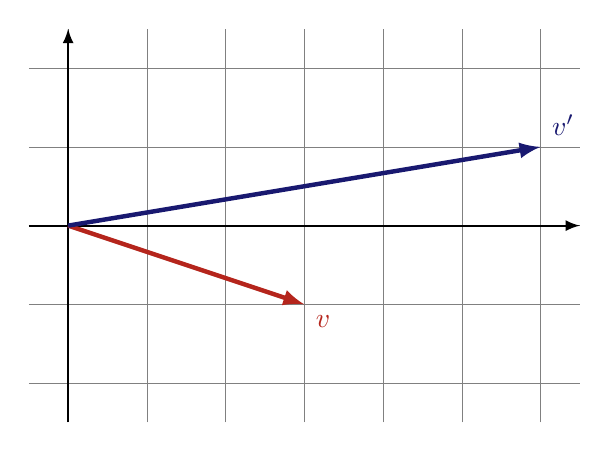
\begin{tikzpicture}
        \draw[step=1, gray,very thin] (-0.5, -2.5) grid (6.5, 2.5);
        \draw[-latex, thick] (0, -2.5) -- (0, 2.5);
        \draw[-latex, thick] (-0.5, 0) -- (6.5, 0);
        \draw[-latex, ultra thick, BrickRed] (0, 0) -- (3, -1) node[below right] {\(v\)};
        \draw[-latex, ultra thick, MidnightBlue] (0, 0) -- (6, 1) node[above right] {\(v'\)};
    \end{tikzpicture}
    \caption{Applying the linear transformation \(M\) to a vector \(v\) produces some other vector \(v'\).}
    \label{fig:Ch11-linear-trans}
\end{figure}

Sometimes, it just so happens that the resultant vector \(v'\) is a scaled version of the original vector \(v'\), i.e.
%
\begin{equation}\label{eq:Ch11-eigen-def}
    v' = Mv = \lambda v
\end{equation}
%
When this happens, the special vector \(v\) is called an \textit{eigenvector} and the corresponding scalar is called its \textit{eigenvalue}. For example, the above matrix has an eigenvector
\(
\begin{pmatrix}
    1 \\ -1
\end{pmatrix}\) because applying the matrix \(M\) to it is equivalent to scaling it by a factor of 3:
%
\[
\begin{pmatrix}
    1 & -2\\
    2 & 5
\end{pmatrix}
\begin{pmatrix}
    1 \\ -1
\end{pmatrix}
=
\begin{pmatrix}
    3 \\ -3
\end{pmatrix}
\]
%
The eigenvalue for this eigenvector is thus 3. See figure \ref{fig:Ch11-eigen}.

\begin{figure}[H]
    \centering
    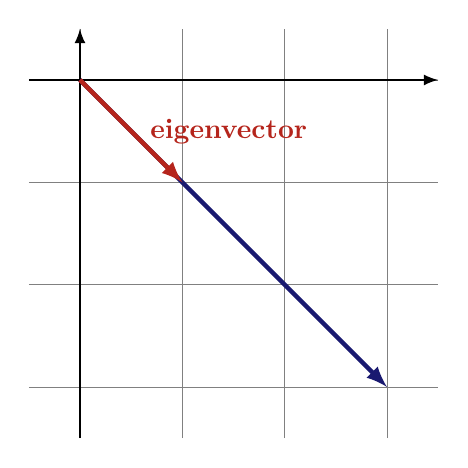
\begin{tikzpicture}[scale=1.3]
        \draw[step=1, gray,very thin] (-0.5, -3.5) grid (3.5, 0.5);
        \draw[-latex, thick] (0, -3.5) -- (0, 0.5);
        \draw[-latex, thick] (-0.5, 0) -- (3.5, 0);
        \draw[-latex, ultra thick, MidnightBlue] (0, 0) -- (3, -3);
        \draw[-latex, ultra thick, BrickRed] (0, 0) -- (1, -1) node[pos=0.5, right] {\;\textbf{eigenvector}};
    \end{tikzpicture}
    \caption{An eigenvector of \(M\) which has an eigenvalue of 3.}
    \label{fig:Ch11-eigen}
\end{figure}

Note that:
%
\begin{itemize}
    \item While the zero vector is technically a solution of \eqref{eq:Ch11-eigen-def}, this is considered a trivial solution (as it is bound to satisfy the equation for any given \(M\)) and is thus excluded from the definition of an ``eigenvector''. 
    \item A matrix can have zero, one or multiple eigenvalues.
    \item If \(v\) is an eigenvector with eigenvalue \(\lambda\), then so is \(kv\) for any nonzero scalar \(k\). This is visualised in figure \ref{fig:Ch11-eigenvalue-has-inf-eigenvectors}.
\end{itemize}

\begin{figure}[H]
    \centering
    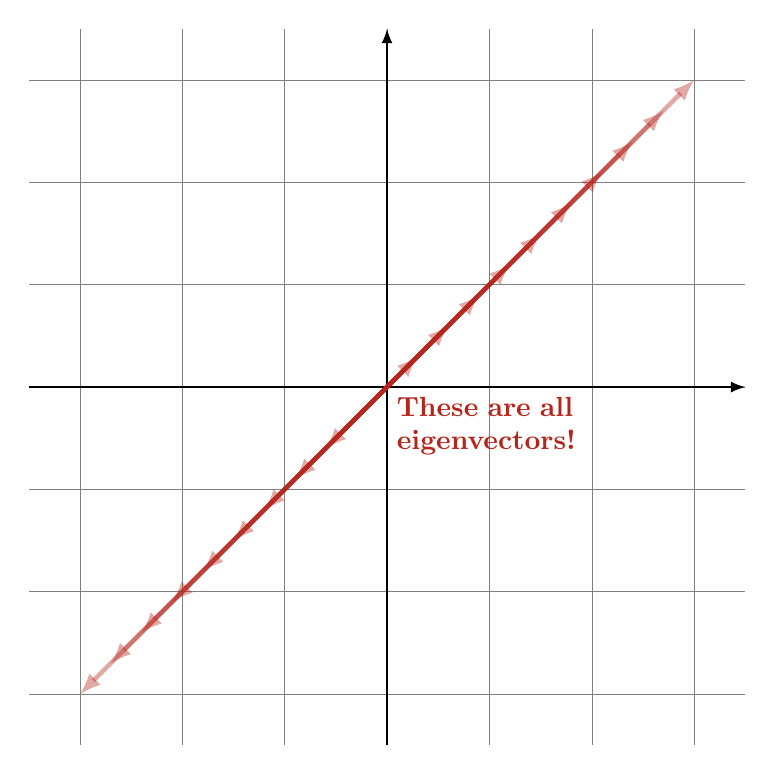
\begin{tikzpicture}[scale=1.3]
        \draw[step=1, gray,very thin] (-3.5, -3.5) grid (3.5, 3.5);
        \draw[-latex, thick] (0, -3.5) -- (0, 3.5);
        \draw[-latex, thick] (-3.5, 0) -- (3.5, 0);

        \foreach \x in {-1,-0.9, ..., -0.1, 0.1,0.2,...,1} {
            \draw[-latex, ultra thick, BrickRed, opacity=0.4] (0, 0) -- (\x*3, \x*3);
        }

        \node[below right, BrickRed, text width=3cm] at (0,0) {\textbf{These are all eigenvectors!}};
    \end{tikzpicture}
    \caption{An eigenvalue corresponds to a line of eigenvectors. (It is also possible for an eigenvalue to correspond to multiple or infinitely many lines of eigenvectors.)}
    \label{fig:Ch11-eigenvalue-has-inf-eigenvectors}
\end{figure}

Given a matrix \(M\), we can compute its eigenvector(s) \(v\) and the corresponding eigenvalue(s) \(\lambda\) by looking for solutions to the following equation.
%
\begin{equation}\label{eq:Ch11-eigen-def2}
    Mv = \lambda v
\end{equation}
%
We do this by rearranging the terms and factoring out \(v\).
%
\begin{align}
    Mv &= \lambda v \notag\\
    Mv - \lambda v &= 0 \notag\\
    Mv - (\lambda I)v &= 0 \notag\\
    (M - \lambda I) v &= 0 \notag\\
    \abs{M - \lambda I} &= 0 \tag{assuming \(v \neq 0\) by definition}
\end{align}
%
Any solution to \(\abs{M - \lambda I} = 0\) would thus give as an eigenvalue, and we can find the corresponding eigenvectors by plugging it into \eqref{eq:Ch11-eigen-def2}.

For a square matrix \(M\) of order \(n \times n\), the expression \(\abs{M - \lambda I}\) is a polynomial of order \(n\) in \(\lambda\). This is known as the \textit{characteristic polynomial} of \(M\). Each eigenvalue of \(M\) is a solution to the equation \(\abs{M - \lambda I} = 0\) (the \textit{characteristic equation}) and is thus a root of the characteristic polynomial. Since the characteristic polynomial has order \(n\), it follows from the fundamental theorem of algebra that \(M\) must have no more than \(n\) eigenvalues.





\subsubsection{Example: A matrix with no eigenvalues}

Consider the matrix
%
\(
R = 
\begin{pmatrix}
    0 & -1\\
    1 & 0
\end{pmatrix}
\).
%
This matrix rotates all vectors counterclockwise by \(90\degree\), so it is intuitively obvious that it should have no eigenvectors whatsoever. To prove this, we construct the following equation.
%
\begin{align*}
    \abs{R - \lambda I} &= 0\\
    %
    \begin{vmatrix}
        -\lambda & -1\\
        1 & -\lambda
    \end{vmatrix} &= 0\\
    %
    \lambda^2 + 1 &= 0
\end{align*}
%
This has no solution, indicating that \(R\) has no eigenvalues (or eigenvectors).




\subsubsection{Example: A matrix with one eigenvalue}

Consider the matrix
%
\(
S = 
\begin{pmatrix}
    1 & 1\\
    0 & 1
\end{pmatrix}
\).
%
(This is called a \textit{shear} mapping.) We calculate its eigenvalues as follows.
%
\begin{align*}
    \abs{S - \lambda I} &= 0\\
    %
    \begin{vmatrix}
        1-\lambda & 1\\
        0 & 1-\lambda
    \end{vmatrix} &= 0\\
    %
    (1-\lambda)^2 &= 0\\
    \lambda &= 1
\end{align*}

We then find the eigenvectors by setting \(v = \begin{pmatrix} x \\ y \end{pmatrix}\).
%
\begin{align*}
    Sv &= 1 \times v\\
    \begin{pmatrix}
        1 & 1\\
        0 & 1
    \end{pmatrix}
    \begin{pmatrix} x \\ y \end{pmatrix} &= \begin{pmatrix} x \\ y \end{pmatrix}\\
    \begin{pmatrix} x + y \\ y \end{pmatrix} &= \begin{pmatrix} x \\ y \end{pmatrix}\\
\end{align*}
%
This gives the following system of equations:
%
\[
\begin{cases}
    x + y = x\\
    y = y
\end{cases}
\]
%
which has the solution \((x, y) = (t, 0)\) for any \(t\). This means that \(S\) has the eigenvectors \(\begin{pmatrix} t \\ 0 \end{pmatrix}\) for any \(t\).



\subsubsection{Example: A matrix with multiple eigenvalues}

Suppose we want to find the eigenvectors for
%
\(
T = 
\begin{pmatrix}
    0 & -6\\
    1 & 5
\end{pmatrix}
\). We again set the following equation:
%
\begin{align*}
    \abs{T - \lambda I} &= 0\\
    \begin{vmatrix}
        -\lambda & -6\\
        1 & 5-\lambda
    \end{vmatrix} &= 0\\
    \lambda^2 - 5\lambda + 6 &= 0\\
    (\lambda - 2)(\lambda - 3) &= 0\\
    \lambda &= 2 \text{ or } 3
\end{align*}
%
We substitute each value of \(\lambda\) into the equation \(Tv = \lambda v\), with \(v\) set to \(\begin{pmatrix} x \\ y \end{pmatrix}\), in order to determine the eigenvectors.

\begin{tabular}{c|c}
    \parbox{0.5\textwidth}{
        For \(\lambda = 2\),
        \begin{align*}
            Tv &= 2v\\
            \begin{pmatrix}
                0 & -6\\
                1 & 5
            \end{pmatrix} \begin{pmatrix}
                x \\ y
            \end{pmatrix} &= \begin{pmatrix}
                2x \\ 2y
            \end{pmatrix}\\
            \begin{pmatrix}
                -6y \\ x+5y
            \end{pmatrix} &= \begin{pmatrix}
                2x \\ 2y
            \end{pmatrix}
        \end{align*}
        %
        This gives the system
        %
        \[
        \begin{cases}
            2x + 6y = 0\\
            x + 3y = 0
        \end{cases}
        \]
        %
        which has the solution
        %
        \[(x, y) = (-3t, t)\]
        %
        or
        %
        \[v = \begin{pmatrix} -3t \\ t \end{pmatrix}\]
        %
        for any \(t\).
    }
    &
    \parbox{0.5\textwidth}{
        For \(\lambda = 3\),
        \begin{align*}
            Tv &= 3v\\
            \begin{pmatrix}
                0 & -6\\
                1 & 5
            \end{pmatrix} \begin{pmatrix}
                x \\ y
            \end{pmatrix} &= \begin{pmatrix}
                3x \\ 3y
            \end{pmatrix}\\
            \begin{pmatrix}
                -6y \\ x+5y
            \end{pmatrix} &= \begin{pmatrix}
                3x \\ 3y
            \end{pmatrix}
        \end{align*}
        %
        This gives the system
        %
        \[
        \begin{cases}
            3x + 6y = 0\\
            x + 2y = 0
        \end{cases}
        \]
        %
        which has the solution
        %
        \[(x, y) = (-2t, t)\]
        %
        or
        %
        \[v = \begin{pmatrix} -2t \\ t \end{pmatrix}\]
        %
        for any \(t\).
    }
\end{tabular}



\subsubsection{The product of all eigenvalues of a matrix equals its determinant}

Here we provide a proof for the following statement:

\begin{quote}
    The determinant of the matrix \(M\) must equal the product of all \(n\) of its eigenvalues.
    %
    \begin{proof}
        Let \(M\) be a square matrix of order \(n\). We know its characteristic polynomial \(P(\lambda) = \abs{M - \lambda I}\) has order \(n\) and has \(n\) (not necessarily distinct) roots \(\lambda_1, \lambda_2, \cdots, \lambda_n\). Each of these \(n\) roots is an eigenvalue of \(M\).
        
        This allows us to express the characteristic polynomial as:
        %
        \begin{equation}\label{eq:char-poly-factored}
            P(\lambda) = k(\lambda - \lambda_1)(\lambda - \lambda_2)\cdots(\lambda - \lambda_n)
        \end{equation}
        %
        where \(k\) is a nonzero constant. By definition, we have:
        %
        \begin{align*}
            \abs{M - \lambda I} &= k(\lambda - \lambda_1)(\lambda - \lambda_2)\cdots(\lambda - \lambda_n)\\
            \begin{vmatrix}
                \boxed{\text{\textbf{?}}} - \lambda & * & \cdots & * \\
                * & \boxed{\text{\textbf{?}}} - \lambda & \cdots & * \\
                \vdots & \vdots & \ddots & \vdots \\
                * & * & \cdots & \boxed{\text{\textbf{?}}} - \lambda \\
            \end{vmatrix}
            &= k(\lambda - \lambda_1)(\lambda - \lambda_2)\cdots(\lambda - \lambda_n)\\
        \end{align*}

        Now consider the \(\lambda^n\) term on both sides.
        %
        \begin{itemize}
            \item On the left hand side, we are trying to compute the determinant of an \(n \times n\) matrix. A \(\lambda^n\) term will only be created when we multiply together the elements on the principal diagonal. Since all principal diagonal elements are of the form \(\left(\boxed{\text{\textbf{?}}} - \lambda\right)\), the determinant's \(\lambda^n\) term must equal \((-\lambda)^n\).

            \item On the right hand side, the \(\lambda^n\) term is \(k \lambda^n\).
        \end{itemize}
        %
        Combining the above gives
        %
        \begin{align*}
            (-\lambda)^n &= k \lambda^n\\
            (-1)^n &= k\\
            k &= (-1)^n
        \end{align*}
        %
        which we can substitute into \eqref{eq:char-poly-factored} to get the following relationship.
        %
        \begin{align*}
            P(\lambda) &= (-1)^n (\lambda - \lambda_1)(\lambda - \lambda_2)\cdots(\lambda - \lambda_n)\\
            \abs{M - \lambda I} &= (-1)^n (\lambda - \lambda_1)(\lambda - \lambda_2)\cdots(\lambda - \lambda_n)
        \end{align*}

        Setting \(\lambda = 0\) yields the following result.
        %
        \begin{align*}
            \abs{M} &= (-1)^n (-\lambda_1)(- \lambda_2)\cdots(- \lambda_n)\\
            &= (-1)^n \left( (-1)^n (\lambda_1 \lambda_2 \cdots \lambda_n) \right)\\
            &= (-1)^{2n} (\lambda_1 \lambda_2 \cdots \lambda_n)\\
            &= \lambda_1 \lambda_2 \cdots \lambda_n \qedhere
        \end{align*}
    \end{proof}
\end{quote}

\vspace{1em}
\hrule
\vspace{1em}


Here is an example problem that makes use of this theorem.

\vspace{1em}
\begin{mdframed}[linewidth=1pt]
\textbf{Problem}

Let \(A\) be a \(3 \times 3\) matrix, whose eigenvalues are \(\lambda_1 = 2\), \(\lambda_2 = 3\) and \(\lambda_3 = 5\).

\begin{enumerate}[label=(\alph*)]
    \item Find the eigenvalues of \(A^2\). Show that the eigenvectors of \(A^2\) are identical to those of \(A\).
    \item Given a positive integer \(n\), express the eigenvalues of \(A^n\) in terms of \(n\). Support your answer with a proof.
    \item Show that \(A\) is invertible.
    \item Find the eigenvalues of \(A^{-1}\). Show that the eigenvectors of \(A^{-1}\) are identical to those of \(A\).
    \item Consider the matrix \(B = A - 5I\). Find the eigenvalues of \(B\) and determine whether \(B\) is invertible.
\end{enumerate}
\end{mdframed}

\vspace{1em}
\begin{mdframed}[linewidth=1pt]
\textbf{Solution}

\begin{enumerate}[label=(\alph*)]
    \item As shown below, the eigenvectors of \(A^2\) are identical to those of \(A\).
    \begin{align*}
        Av &= \lambda v\\
        A^2 v &= A (\lambda v)\\
        A^2 v &= \lambda (A v) \\
        A^2 v &= \lambda (\lambda v) \\
        A^2 v &= \lambda^2 v
    \end{align*}
    %
    The last line shows that the eigenvalues of \(A^2\) are the squares of those of \(A\), i.e. 4, 9 and 25.
    
    \item The eigenvalues of \(A^n\) are \(2^n\), \(3^n\) and \(5^n\).

    \begin{proof}
        We proceed by induction. The base case is established by the fact that for \(n = 1\), the matrix \(A^n = A^1 = A\) has the eigenvalues \(\lambda = 2, 3, 5\), i.e. \(Av = \lambda v\).

        Now assume that for some positive integer \(k\), the eigenvalues of \(A^k\) are \(\lambda^k = 2^k, 3^k, 5^k\). It follows that
        %
        \begin{align*}
            A^k v &= \lambda^k v \tag{induction hypothesis}\\
            A \left(A^k v \right) &= A \left(\lambda^k v\right)\\
            A^{k+1} v &= \lambda^k (Av)\\
            A^{k+1} v &= \lambda^k (\lambda v) \tag{base case}\\
            A^{k+1} v &= \lambda^{k+1} v
        \end{align*}
        %
        which completes the induction step.
    \end{proof}

    \item \(\abs{A} = 2 \times 3 \times 5 = 30 \neq 0\), so \(A\) is invertible.
    
    \item As shown below, the eigenvectors of \(A^{-1}\) are identical to those of \(A\).
    \begin{align*}
        Av &= \lambda v\\
        A^{-1} A v &= A^{-1} (\lambda v)\\
        v &= \lambda (A^{-1} v) \\
        A^{-1} v &= \frac{1}{\lambda} v
    \end{align*}
    %
    The last line shows that the eigenvalues of \(A^{-1}\) are the reciprocals of those of \(A\), i.e. \(1/2\), \(1/3\) and \(1/5\).
    
    \item Again, the eigenvectors of \(B = A - 5I\) are identical to those of \(A\).
    %
    \begin{align*}
        Av &= \lambda v\\
        Av - 5v &= \lambda v - 5v\\
        (A-5I) v &= (\lambda - 5) v\\
        B v &= (\lambda - 5) v\\
    \end{align*}
    %
    The last line shows that the eigenvalues of \(B\) are simply \(\lambda - 5\), i.e. \(-3\), \(-2\) and \(0\). The determinant of \(B\), which is the product of the eigenvalues, is 0. This implies that \(B\) is not invertible.
\end{enumerate}
\end{mdframed}




